\documentclass[12pt, a4paper]{article}
\usepackage[a4paper, margin=2.5cm]{geometry}
\usepackage[utf8]{inputenc}
\usepackage[english]{babel}
\usepackage{graphicx}
\usepackage{setspace}
\usepackage{parskip}
\usepackage[htt]{hyphenat}
\usepackage[labelsep=period, labelfont=bf, textfont=it, skip=5pt]{caption}

\usepackage{chngcntr}
\counterwithin{figure}{section}

\usepackage[style=apa, citestyle=apa]{biblatex}
\addbibresource{bibliography.bib}

\graphicspath{ {images/} }

\begin{document}

\begin{titlepage}
	\begin{center} 
		
\includegraphics[width=0.8\textwidth]{nti_kronhus}
		\vfill 
		\Huge
		An internet client library in C++20\vspace{1.5em}\\
		Ett internetklient-bibliotek i C++20
	\end{center}
	\vfill 
	\setstretch{1.5}
	\textbf{Elev: }Björn Sundin\\
	\textbf{Handledare: }Victor Frealdsson\\
	\textbf{Program: }Teknik\\
	\textbf{År: }2020-2021
\end{titlepage}

\section*{Preface}
The student is currently attending the technology program at NTI-gymnasiet Kronhus. The technology program is university preparatory and includes, among many others, technical subjects such as programming, higher-level mathematics, and physics.

My interest in programming started when I was 13 years old and I first learned the basics of C++ and JavaScript. My first project was programming an RPG game in C++ with my best friend Noah who is an artist, music writer/producer, and animator. In later years, my interest in C++ has grown quite large. I have been digging into all of the details and quirks of the language as well as learned about the features and changes of newer standards.

There are six published C++ ISO standards as of today; C++98, 03, 11, 14, 17, and 20. C++11 was a major update with many new features and improvements that changed the way we wrote code. C++20 is the most recent standard and was published only a few months ago as this is written. This new standard is said to potentially have an even bigger impact on the language. 

Learning about all of these new features made me curious and gave me the idea to start this project at the beginning of the school year; a library written from the ground up in C++20, taking advantage of as many new features and techniques as possible. I chose HTTP requests because I had tried a couple of existing libraries for this but was disappointed in their designs and user interfaces (in terms of code; not graphical).

The majority of this work can be read with no knowledge or experience with C++, but some knowledge of programming and general programming terminology is expected. Some parts of section \textbf{\ref{sec:Results}} are targeted towards readers that have more knowledge of C++ or are willing to do some further reading, as it discusses features of the language in more detail and it is beyond the scope of this text to teach the language. I have tried to refer to pages on CppReference and similar resources where interested readers may read further on the topics.

I would like to thank my best friends and creative souls Noah and Linnéa for being there throughout the years and giving me motivation.

\clearpage
\section*{Abstract}
This report describes and discusses the development of a piece of software written in the C++20 programming language. The software is a high-level library for sending and receiving data over the internet, primarily over the HTTP protocol. The purpose is firstly to explore how taking advantage of features and changes in newer C++ standards can affect software development in practice. A second purpose is to discuss the usage and effects of different best practices, design principles, and programming paradigms in relation to the project. Another issue that the work explores is unit testing and how good test coverage can be accomplished through design.\medskip

The library has specific design goals and restrictions that are presented in the introduction. To give background and context to the project, similar existing works are compared to the idea for this work. The software development process is then described from start to finish and the results presented in terms of the resulting library structure and usage. The most significant results of this work are in the discussion, where topics such as the usage of programming paradigms, modern C++ features, design concerning testability, performance, safety, and error handling are reviewed and examined in relation to the project and with more general conclusions.

\clearpage
\tableofcontents

\clearpage
\section{Introduction}

\subsection{Idea}\label{sec:Idea}
The idea is to write a modern library in C++20 for easily making secured and unsecured HTTP requests. 

Some specific aims with the library are:
\begin{itemize}
	\item A user-friendly, functional design.
	\item An API that is hard to misuse.
	\item The code follows the C++ Core Guidelines (\cite{CppCoreGuidelines}).
	\item Lightweight with minimal dependencies.
	\item Support for asynchronous requests.
	\item Support for callbacks for inspecting and/or canceling responses while they are being received.
	\item Support for Windows, MacOS, and Linux operating systems.
	\item Free from compiler warnings with all useful C++ warning flags turned on.
	\item Modern CMake integration.
\end{itemize}

\subsection{Purpose}
The purpose of this project was originally to explore how modern language and library features introduced in C++17 and C++20 can affect software and its development in practice. Another purpose is to explore techniques in software development for the abstraction of low-level APIs. Different programming paradigms, design principles, and best practices are discussed in relation to the development of the project.
\subsection{Questions to answer}

\begin{itemize}
	\item The library is a set of high-level abstractions on top of low-level APIs. Which APIs are most fitting to build the abstractions from?
	\item The goal of the project is to design robust interfaces that are hard to misuse. Which language/library features, principles, and paradigms can be used to accomplish this?
	\item To ensure that the code is correct and that changes do not break the intended behavior of interfaces, the code needs to be testable. What are ways to design the code to accomplish good test coverage?
\end{itemize}

\subsection{Demarcation}
Only the HTTP protocol is supported, other protocols like FTP are not implemented. Not all advanced HTTP features are implemented. Only HTTP/1.1 is supported.

\clearpage
\section{Background}
\subsection{Previous works}
\subsubsection{cpr}
cpr is an HTTP request library written as an abstraction on top of the popular C library libcurl (\cite{Cpr}). The description on their GitHub page is: “C++ Requests: Curl for People, a spiritual port of Python Requests”.

\begin{itemize}
	\item cpr provides most of the functionality that Cpp20InternetClient aims to provide.
	\item According to the README.txt file on their GitHub page, cpr requires OpenSSL for making HTTPS requests. OpenSSL is an API mainly for SSL/TLS encryption and decryption (\cite{OpenSSL}). A goal of Cpp20InternetClient is to reduce the need for these kinds of dependencies as much as possible, automatically making use of Windows-native APIs on the Windows operating system. 
	\item cpr is built on top of libcurl, a mature C library for making many different types of internet requests (\cite{Libcurl}). This has the advantage of making the core functionality stable and trusted by users. However, libcurl is a very big and old library that contains much more than what Cpp20InternetClient aims to support. This project has the aim of being lightweight and having minimal dependencies. Additionally, interacting with less user-friendly, native APIs and implementing more functionality ourselves gives more opportunities to discuss interesting uses of new language features and modern programming practices.
	\item cpr is written in the C++11 programming language standard and therefore does not make use of newer language features and improvements introduced in C++14, C++17, and C++20.
	\item Making simple HTTP requests using cpr requires little code and is expressive. The function used to create GET requests is a variadic template that takes any number of parameters for passing things like the URL, request headers, and authentication parameters. These parameters can be passed in any order. See \textbf{Figure \ref{fig:cpr_example}} for an example GET request.

	These variadic template functions are however easy to use incorrectly, as the function declaration says nothing about what types the parameters are required to be. When an object of an unsupported type is passed as one of the parameters to the function, the code still compiles, but \texttt{cpr::Get} returns an empty response. An example of code that fails silently in such a way is shown in \textbf{Figure \ref{fig:cpr_example_incorrect}}. It is not apparent from the user’s perspective what went wrong. A goal of Cpp20InternetClient is to make interfaces hard to misuse and easy to use correctly, while at the same time hiding low-level details and being expressive. As many errors as possible should be caught at compile time.
	\item cpr is not free from many of the useful warning categories provided by compilers like GCC, and can therefore not be built with the -Werror flag (\cite{GccWarnings}). A goal of Cpp20InternetClient is to compile with -Werror and all useful warning flags turned on.
\end{itemize}

\begin{figure}[hp]
	\centering
	\caption{Example of a GET request with cpr. The fmt library is used for formatted text output.}
	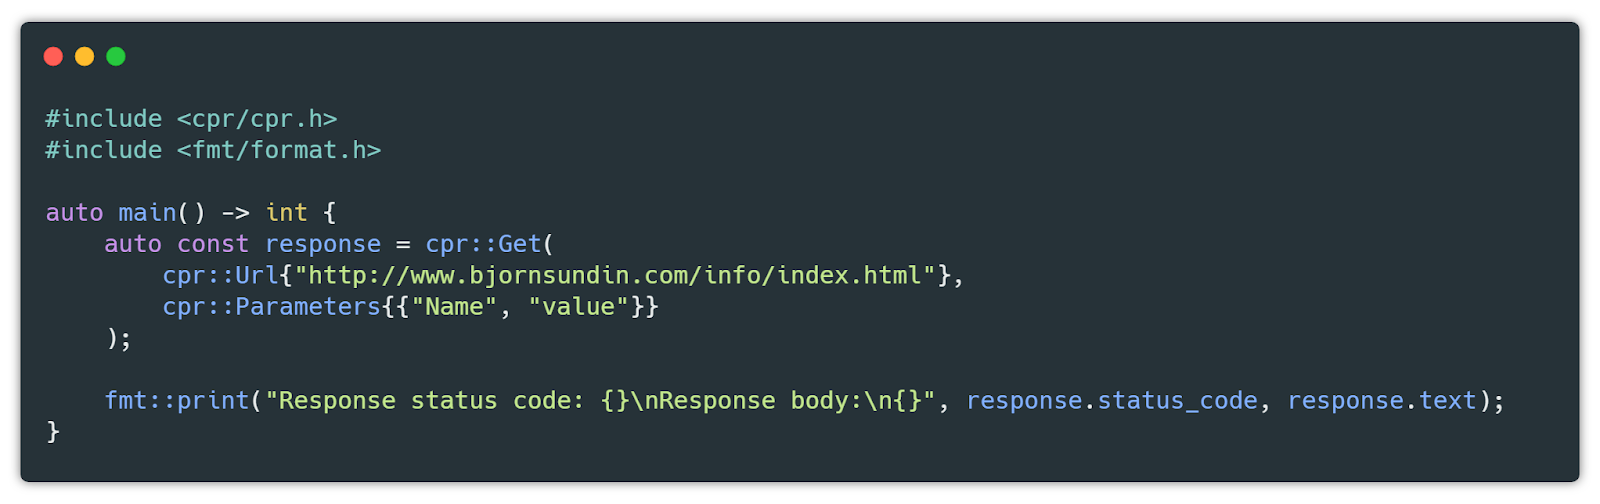
\includegraphics[width=\textwidth]{cpr_example}
	\label{fig:cpr_example}
\end{figure}

\begin{figure}[hp]
	\centering
	\caption{Example of a GET request with cpr, written incorrectly. This code fails silently and prints an empty response body and a status code of 0.}
	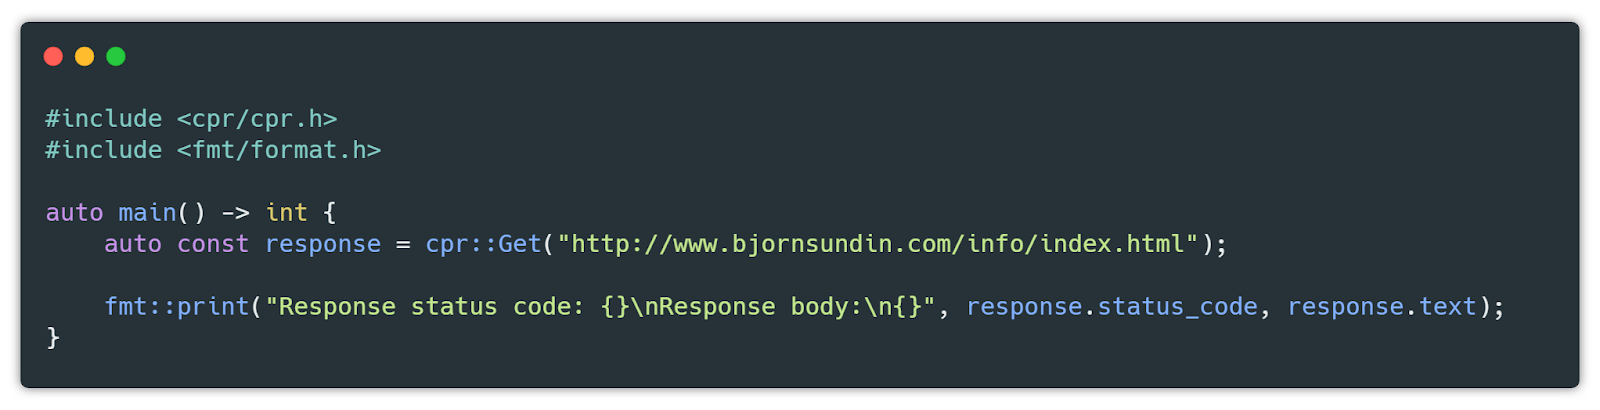
\includegraphics[width=\textwidth]{cpr_example_incorrect}
	\label{fig:cpr_example_incorrect}
\end{figure}

\subsubsection{Boost.Beast}
Boost is a set of header-only C++ libraries. Boost.Beast one of these and provides “low-level HTTP/1, WebSocket, and networking protocol vocabulary types and algorithms using the consistent asynchronous model of Boost.Asio” (\cite{BoostBeast}). Boost.Asio is a Boost library for low-level network I/O (\cite{BoostAsio}).
\begin{itemize}
	\item Boost.Beast provides most of the functionality that Cpp20InternetClient aims to provide.
	\item The library requires OpenSSL for TLS encryption, and like cpr does not take advantage of native Windows APIs.
	\item Because Boost.Beast is header-only, all of its dependencies are leaked into the global namespace when including the headers, such as the OpenSSL API. Our library will only expose its own API and hide any dependencies in its own translation unit since unwanted names can cause problems.
	\item The abstraction level of Boost.Beast is relatively low. This means that it is easy to make mistakes in the process of writing code to perform an HTTPS request for example. See \textbf{Figure \ref{fig:boost_beast_example}} for an example of performing a GET request over HTTPS using Boost.Beast. An advantage with this low level of abstraction however is that it allows for a great level of customization, and abstractions can be built on top of it. In this work, we focus more on ease of use and safety than on being able to have fine-grained control over details, while still being useful for the most common cases.
	\item Boost.Beast is written in C++11 and does not take advantage of newer library and language features introduced in C++14, C++17, or C++20.
	\item Boost.Beast is free from warnings when compiled by GCC, which is something this project aims to be as well.
\end{itemize}

\begin{figure}[hp]
	\centering
	\caption{Example of a “GET” HTTPS request using Boost.Beast.}
	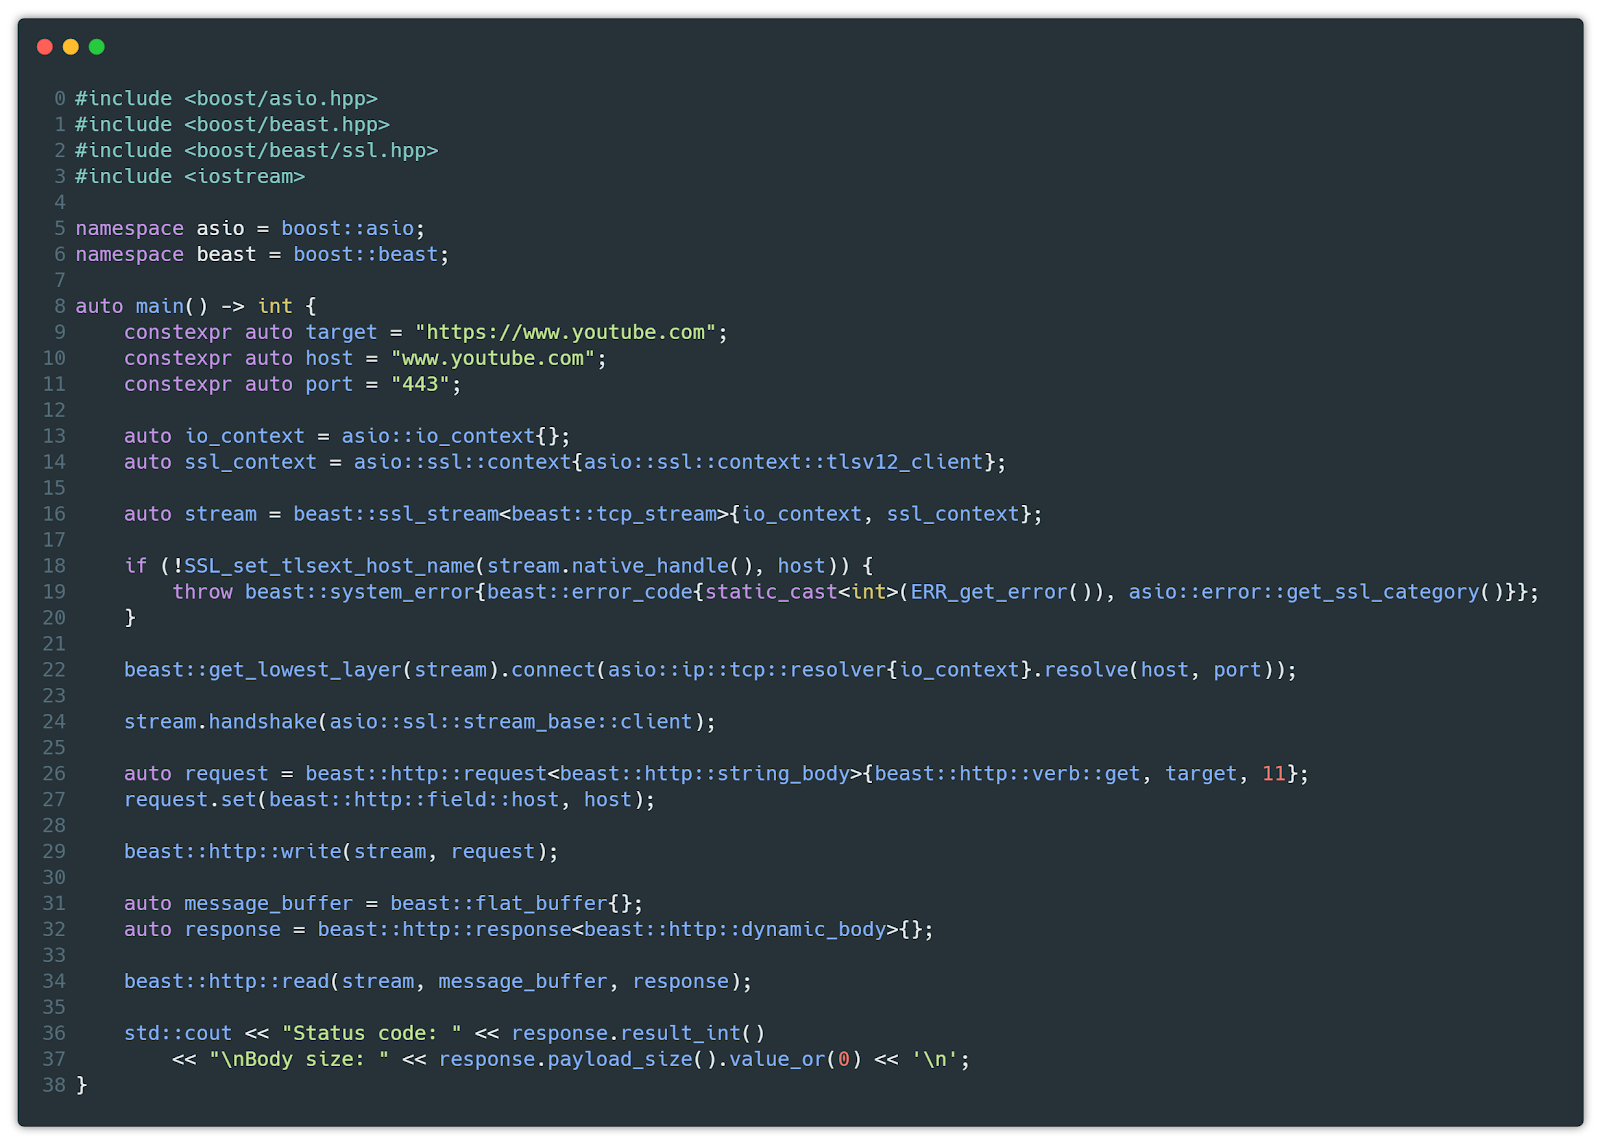
\includegraphics[width=\textwidth]{boost_beast_example}
	\label{fig:boost_beast_example}
\end{figure}

\clearpage
\subsection{Concepts and definitions}
\subsubsection{Cpp20InternetClient}
The name that is used to refer to the project in the text. It is also the name of the CMake package namespace.

\subsubsection{I/O stream}
Something that can both send and receive binary data. This can be a socket, a file, a console user interface, etc.

\subsubsection{POSIX}
A family of standards that define APIs of UNIX-like operating systems (which include Linux and MacOS) (\cite{Posix}). An example of an API that POSIX defines is the POSIX socket API.

\subsubsection{Object files}
An object file is what a C++ compiler outputs and what the linker uses as input (\cite{UnderstandingCompilation}). The compiler compiles every translation unit into a binary object file, and the linker links these together, “filling in” any references to compiled code (function addresses) in other object files, and outputting a complete executable or library.

\subsubsection{Header files and translation units}
A C++ header file usually has the extension \texttt{.h} or \texttt{.hpp} and contains C++ code that the preprocessor can copy into other C++ files, whether they are other header files or implementation files (\cite{UnderstandingCompilation}). This is done through the preprocessor directive \texttt{\#include}, which tells the preprocessor to copy the contents of the specified header file into the file that includes it. The preprocessor is a program that is run before any actual compilation of C++ code begins. The output from the preprocessor and input to the compiler is a translation unit.

\subsubsection{Implementation files}
This is a C++ source file, usually with the extension \texttt{.cpp}, that contains code that corresponds to one translation unit and is compiled to an object file. An implementation file can \texttt{\#include} header files.

\subsubsection{SSL/TLS}
TLS is a protocol for encryption and decryption of data sent over the internet, providing communication security (\cite{TlsSpec}). HTTPS is HTTP encrypted using TLS. SSL is the predecessor of TLS.

\subsubsection{TLS handshake}
The first step in establishing a secure connection over TLS is performing a handshake (\cite[][Section 4]{TlsSpec}). In this process, different security parameters are negotiated between the client and the server.

\subsubsection{Buffer}
A buffer is a block of data in memory, consisting of an often large number of bytes (eight bits each). Buffers are used to hold arbitrary data that some part of the program can understand and manipulate for some specific purpose. For example, an image can be stored in a buffer.

\subsubsection{HTTP message headers}
The headers of an HTTP message comprise a list of (name, value) pairs that provide various types of structured information to the server or client (\cite[][Section 4.2]{HttpSpec}). An example is the \texttt{Content-Length} header that indicates the size of the message body in bytes (Section 14.13).

\subsubsection{HTTP message body}
The body of an HTTP message carries any data that is sent to the server or client (\cite[][Section 4.3]{HttpSpec}). The type of message body data can be specified with the \texttt{Content-Type} header (Section 14.17). For example, the contents of an HTML document can be carried in the body of an HTTP response message.

\clearpage
\section{Method}
\subsection{Research methods}
Documentation and specifications were referred to when implementing protocols and using APIs. Two primary sources that were used during the development process were Microsoft’s API documentation (\cite{MicrosoftDocs}) and CppReference (\cite{CppReference}). Other sources of information were the HTTP/1.1 specification (\cite{HttpSpec}) and the TLS 1.3 specification (\cite{TlsSpec}). The book \citetitle{ModernCMakeBook} (\cite{ModernCMakeBook}) was used as a resource for learning to write modern CMake. The CMake reference documentation (\cite{CMakeReference}) was referred to as well. The developer forum StackOverflow (\cite{StackOverflow}) was used occasionally for guidance on some issues that arose. 

One of the aims of this project was, as mentioned in \textbf{\ref{sec:Idea}}, to follow the C++ Core Guidelines (\cite{CppCoreGuidelines}), which are “[...] a set of guidelines for using C++ well.”. These guidelines are an open source, living document created and maintained by Bjarne Stroustrup, who is the creator of C++, and Herb Sutter, a prominent C++ expert. Large portions of this document were read before the development of the library and were kept in mind during development in an attempt to apply the guidelines to the code.

Inspiration was taken from presentations from Cppcon (\cite{CppCon}) as well as from YouTube videos by Jason Turner (\cite{JasonTurnerChannel}). The presentation \citetitle{MattGodboltCorrectByConstruction} by Matt Godbolt (\cite{MattGodboltCorrectByConstruction}) from the “C++ on Sea” conference was also a big inspiration and source of information.

\subsection{Work process}
The work consisted entirely of concurrently doing research, designing, and programming. The details of this are discussed in the following section.

\subsection{Software development process}
The work was initiated by laying out an initial directory structure, creating a single header file and implementation file for the library code, and adding a small usage concept code snippet as shown in \textbf{Figure \ref{fig:concept_snippet}}. Starting this way was inspired by the test-driven development technique where test code that checks the correctness of modules is written before the implementation of the functionality (\cite{TestDrivenDevelopment}). The technique can be beneficial because it gives the programmer a clear goal of what the code is required to do and what the interface will look like. As a result, the implementation can be simplified and refactored without worrying about breaking anything from the perspective of the user, since the tests check that the code is correct. 

Another example of a (non-strict) application of this technique in the project was the writing of unit tests and usage of a unit testing framework. A unit test is a piece of code that checks the correctness of some functionality. The idea is that the code should be designed such that every component can be tested individually, making bugs quicker to find and improving the stability of whole programs that use these components. The unit testing framework Catch2 was chosen for this project. Catch2 is header-only, relatively small, and written using modern C++ features up until the latest standard (\cite{Catch2}). Catch2 is the second most used C++ unit testing framework, behind Google Test (\cite{DeveloperStatistics}). The single-header version of the framework was added to the project and a subdirectory for tests was created. 

To build the library, unit tests, and example programs, some kind of build system was needed since running a compiler and linker manually is unsustainable. There are many different build systems, some of which are system-dependent. Two examples of system-dependent build systems with support for C++ are MSVC build tools and XCode. These build systems are targeted towards specific operating systems, compilers, and linkers. To support multiple build systems, a build generator was used. The most used build generator for C++ projects is CMake (\cite{DeveloperStatistics}). Using CMake as the build generator was advantageous because it also has a package integration system that allows for simple installation and usage of libraries. Since it is the most widely used build generator, Cpp20InternetClient will be able to integrate easily with a larger quantity of C++ projects. A simple CMake configuration script was written to generate builds of the library, the initial concept program in \textbf{Figure \ref{fig:concept_snippet}} as well as of the unit testing program.

\begin{figure}[hp]
	\centering
	\caption{Initial concept code snippet. This was later developed into a more detailed code example for making a GET request using the library. Note that the name of the library header has changed since then.}
	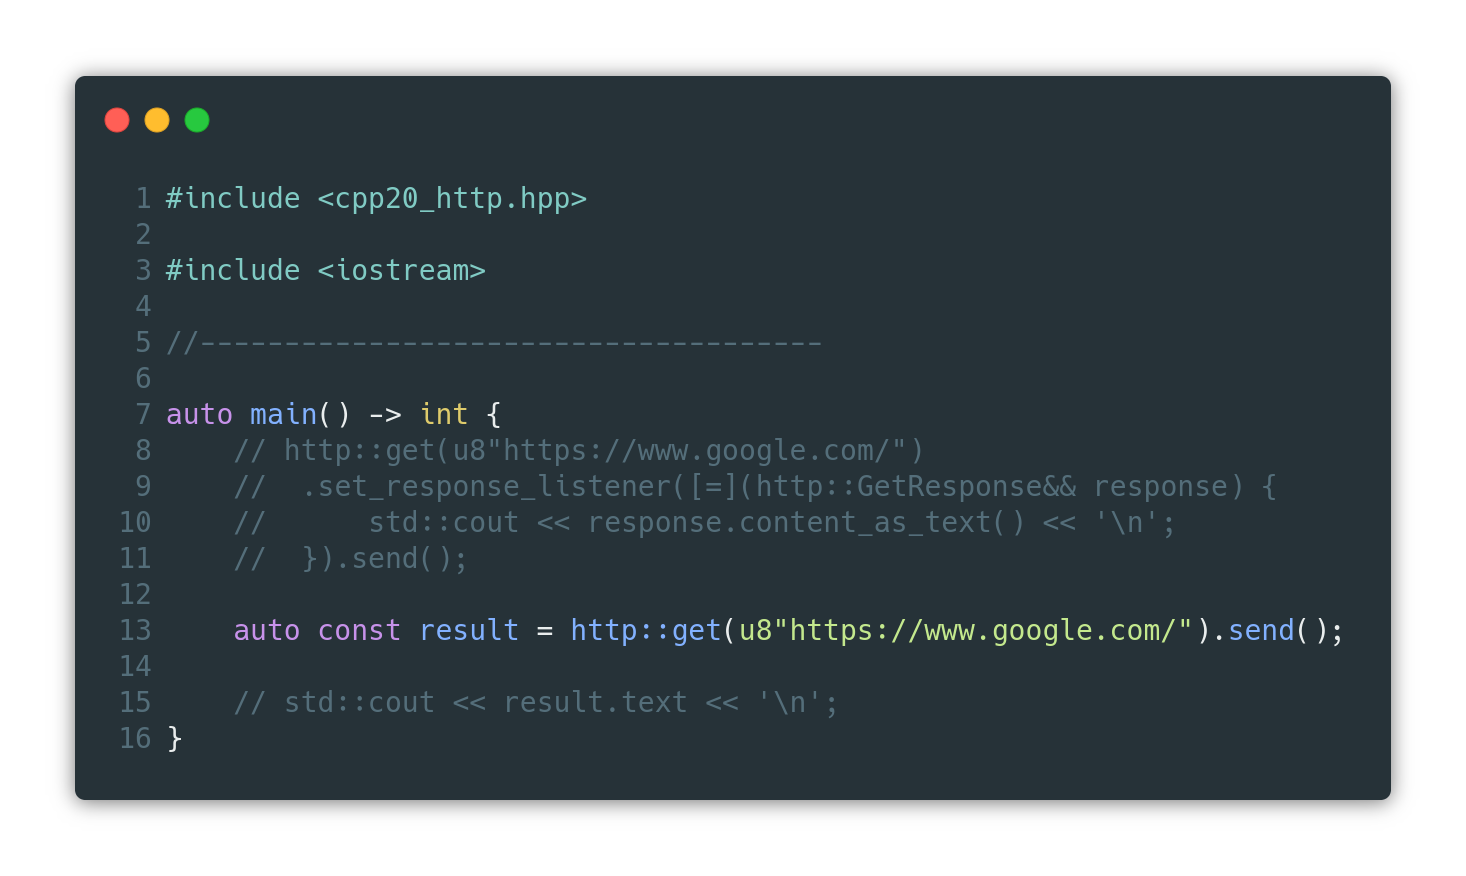
\includegraphics[width=\textwidth]{concept_snippet}
	\label{fig:concept_snippet}
\end{figure}

The first functionality that was implemented was the ability to send a GET request over unsecured HTTP, blocking and returning the received response headers and body. The initial development of the library was done on the Windows operating system. Thus, a native Windows API was chosen to provide the most low-level functionality that the library abstracts, assuming there was a corresponding API on Linux and MacOS systems. The first implementation of the mentioned functionality was built on top of an API named WinINet. WinINet provides a full implementation of FTP, HTTP/1.0 and HTTP/1.1 (\cite{MicrosoftWinINet}). 

However, it turned out that there is no corresponding C or C++ API on Linux and MacOS. After this first working implementation of simple GET requests and responses was finished, the majority of the code was rewritten to make use of a lower-level API that all of the targeted operating systems support equivalent versions of. A class was written that abstracts the only needed platform-dependent functionality; a TCP socket. A socket only provides an I/O interface to a remote computer, in this case, a server. This meant that the HTTP implementation had to be written from scratch.

The PImpl (“Pointer to Implementation”) idiom (\cite{CppPImplIdiom}) was used to separate Windows API and POSIX-based implementations of the \texttt{Socket} abstraction. In the PImpl idiom, the interface class (that is declared in the header file and the user interacts with) contains a private forward declaration (\cite{CppClassDeclaration}) of an implementation class and a \texttt{std::unique\_ptr} that holds an instance of the implementation. \textbf{Figure \ref{fig:pimpl_forward_declaration}} shows what this looks like. This made it possible to write different classes for different implementations of the same functionality, keeping only function declarations in the header file and defining them in the implementation file by forwarding the calls to the inner implementation class instance. Note that this is different from just declaring member functions in a header file and defining them in the implementation file. In the PImpl idiom, the implementation has its own whole class with its own members.

\begin{figure}[hp]
	\centering
	\caption{Shows the most important part of the PImpl idiom in the interface class; a forward declaration of an implementation class and a dynamically allocated instance of it.}
	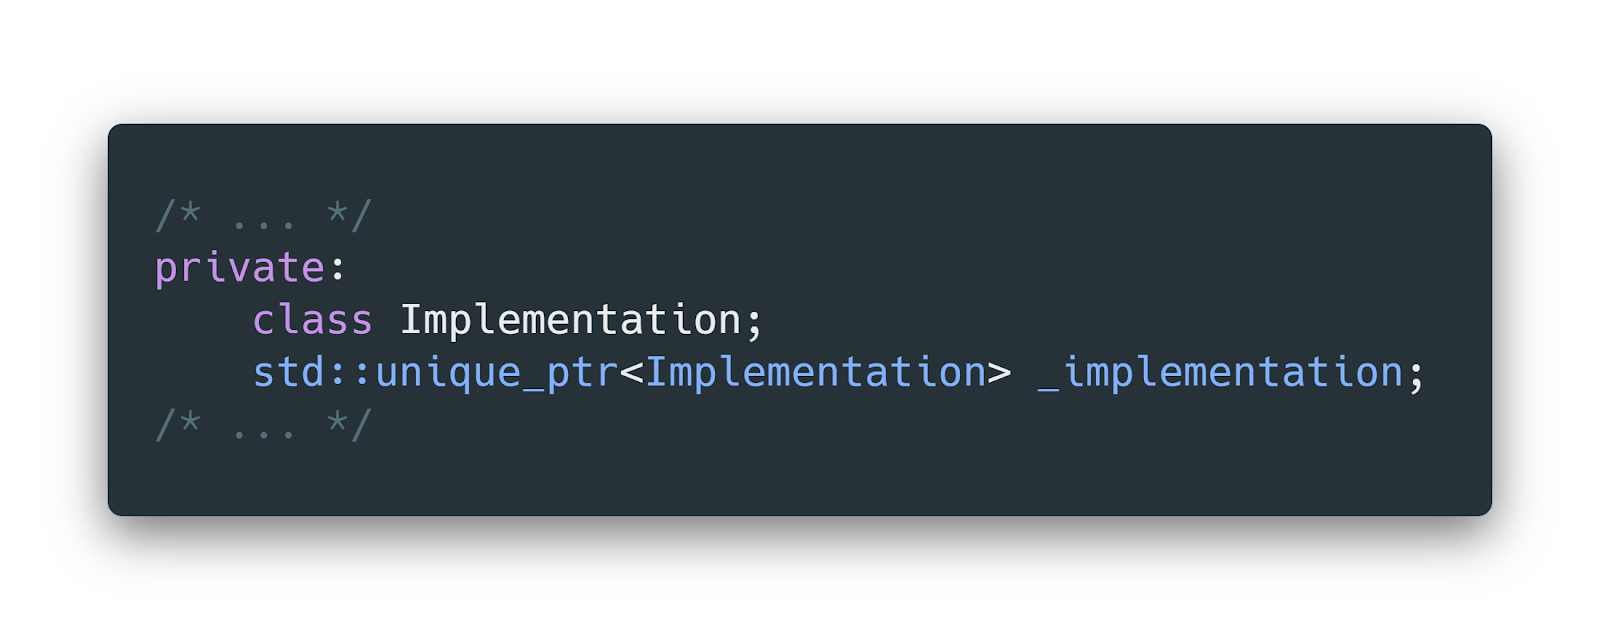
\includegraphics[width=0.8\textwidth]{pimpl_forward_declaration}
	\label{fig:pimpl_forward_declaration}
\end{figure}

Between HTTP and TCP/IP there can also be a layer of encryption, like TLS (Transport Layer Security). HTTP that is encrypted using TLS or its older version SSL is called HTTPS (\cite{HttpsGlossary}). Once the unencrypted socket implementations were finished, an option for TLS encryption had to be added to the \texttt{Socket} class for HTTPS support. The Windows Schannel API was used for this on Windows, and OpenSSL was used on Linux and MacOS. Instead of having two different definitions of the implementation class (\texttt{Socket::Implementation}), one for Windows sockets and one for POSIX sockets, the functionality was moved into a separate class in the implementation file, \texttt{RawSocket}. This was done to better separate the functionality when TLS encryption was added; a \texttt{TlsSocket} class was written (also with two implementations for the different platforms) that is built on top of \texttt{RawSocket}, only adding the layer of TLS encryption. Then, \texttt{Socket::Implementation} only has to hold a \texttt{std::variant<RawSocket, TlsSocket>} that either holds a \texttt{RawSocket} or \texttt{TlsSocket}, forwarding the function calls depending on the type.

HTTP was implemented in the header file to allow for maximum compiler optimization and template parameterization in multiple translation units. The namespace \texttt{internet\_client::http} was added to contain the HTTP types and functions provided to the user, and \texttt{http::algorithms} to contain types and functions for separating the responsibilities of the implementation of those interfaces (mainly different parsing algorithms). Some examples of these components are \texttt{parse\_status\_line} for parsing HTTP response status lines and \texttt{ChunkyBodyParser} for parsing response body data sent with the “chunked” \texttt{transfer-encoding} (\cite{HttpTransferEncoding}). These were not meant for use by other programs, although they could be, and there is no danger in using them. Tests were written for each component of the HTTP implementation.

Support for callbacks and asynchronous requests was implemented and more HTTP request types were added, for example, “POST”. Multiple example programs were written to perform different types of requests in different ways. Toward the end of the development process, the CMake script was extended to allow for installation and easy integration with other CMake projects.

The library was tested on Windows, MacOS, and Linux. The Windows system was Windows 10 on an internal SSD on a laptop. The Linux system used was Ubuntu version 20.04 and 20.10, on an external SSD booted on the same laptop. The MacOS version was Catalina 10.15.5, on a virtual machine ran on the Ubuntu system using VirtualBox virtualization software.

\clearpage
\section{Results}
The results presented here are based on version 2.1.0 of the library. The code for this version can be found in the GitHub repository (\cite{Cpp20InternetClient}). The library itself consists of 3244 lines of C++ code and the unit tests consist of 577 lines of code. At the time of its release, it could only be compiled by GCC version 10.2.0 or later, not Clang or MSVC. This was because C++20 features were used that the other compilers had yet to implement.
\subsection{Library structure}
The final directory structure of the project can be seen in \textbf{Figure \ref{fig:directory_structure}}. Below is a description of what each directory contains.
\begin{enumerate}
	\item \textbf{cmake} - This contains a single file, \texttt{Cpp20InternetClientConfig.cmake.in}. This is a CMake script that only has the purpose of finding the dependencies of the library during installation.
	\item \textbf{examples} - These are example programs that use the library to perform different types of HTTP requests using different features of the library. They can be seen as integration tests and as help to other developers wishing to use the library.
	\item \textbf{external} - This contains smaller dependencies of the library, in this case only the Catch2 unit testing framework header.
	\item \textbf{include} - Contains the C++ header to be included by programs and by the implementation file.
	\item \textbf{source} - Contains the C++ implementation file to be built as a static library to be linked to by programs using the library. Only code that depends on external library headers is implemented in this file.
	\item \textbf{tests} - Contains all of the unit tests for the library. Each file contains one or more unit tests that test a class or function of the library. \texttt{test\_main.cpp} is a file containing the entry point of the unit testing program.
\end{enumerate}

\begin{figure}[hp]
	\centering
	\caption{The final directory structure of Cpp20InternetClient.}
	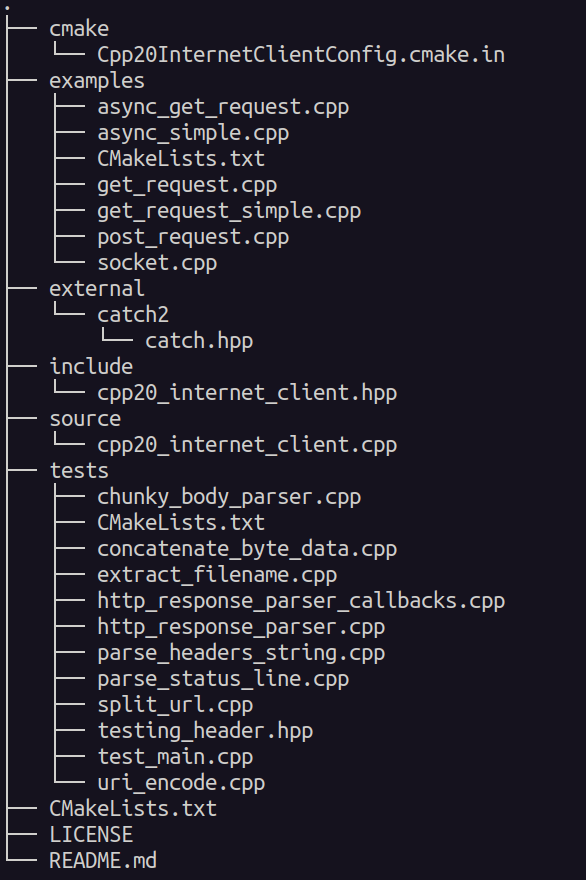
\includegraphics[width=0.7\textwidth]{directory_structure}
	\label{fig:directory_structure}
\end{figure}

The library consists of the namespaces outlined below:

\begin{verbatim}
internet_client {
    errors
    http {
        algorithms
    }
    utils
}	
\end{verbatim}

errors contains types that can be thrown by functions in the library and caught by the user; for example \texttt{ConnectionFailed}. \texttt{http} contains everything related to the HTTP protocol specifically; for instance, \texttt{Socket} falls outside of this namespace. algorithms contains all of the lower-level HTTP-related modules that are not expected to be used directly by the user; for example \texttt{ChunkyBodyParser}. \texttt{utils} contains general utilities that are used by the library. Some of them might be useful for users as well; for example \texttt{write\_to\_file}.
\subsection{Library usage}
Only two examples of library usage are shown here, and not all provided functionality is demonstrated due to space and time constraints. Refer to the “examples” directory in the GitHub repository (\cite{Cpp20InternetClient}) for more usage examples.

\textbf{Figure \ref{fig:get_request_example}} shows a simple example of a blocking (synchronous) GET request with a custom header field passed as a \texttt{http::Header} object and writing the body to a file named “\texttt{response\_image.jpg}”. Any connection errors are handled by printing a description of the error. The output file of the program is shown in \textbf{Figure \ref{fig:get_request_output}}. Possible console output from the program in case there is no internet connection is for instance:
\begin{verbatim}
    The connection failed - "Failed to get address info for socket 
    creation: Temporary failure in name resolution"
\end{verbatim}

\begin{figure}[hp]
	\centering
	\caption{Example library usage to perform a simple HTTP “GET” request.}
	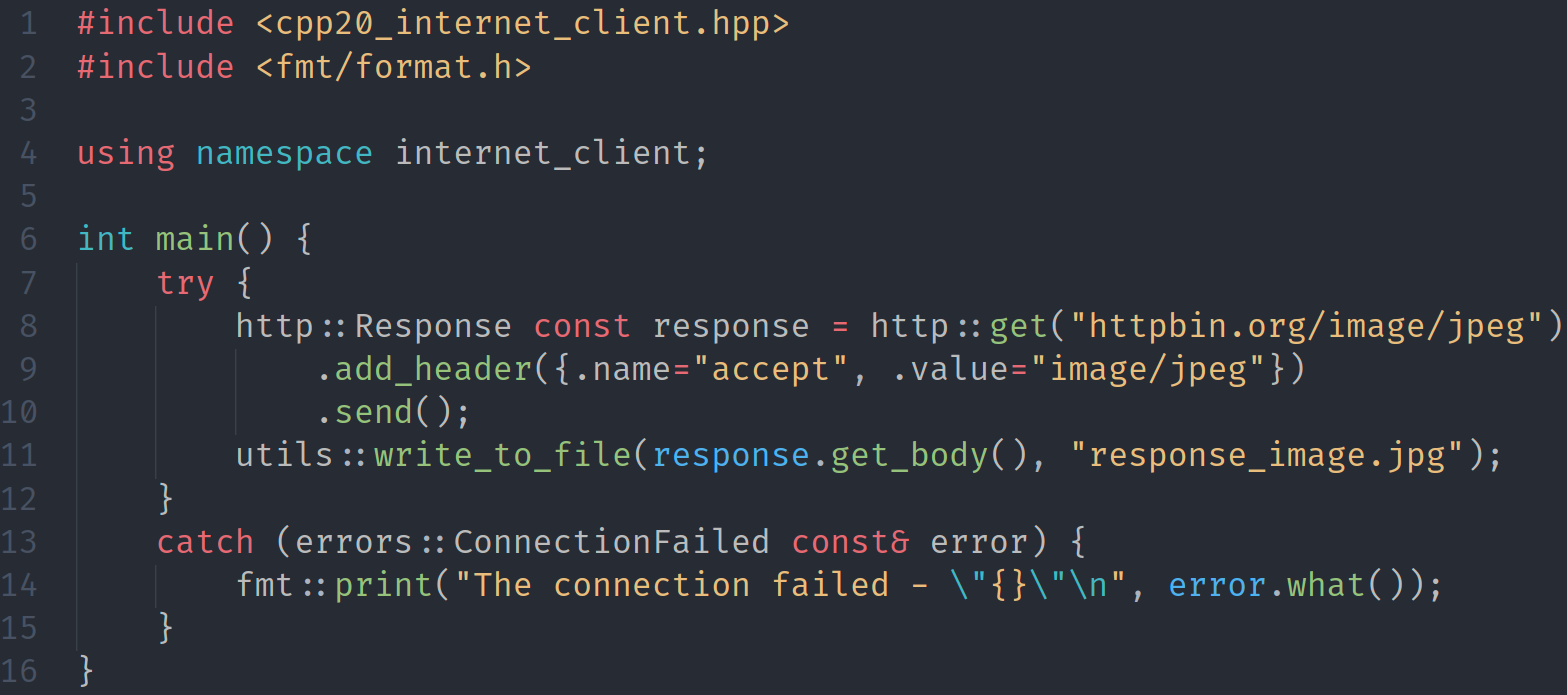
\includegraphics[width=\textwidth]{get_request_example}
	\label{fig:get_request_example}
\end{figure}

\begin{figure}[hp]
	\centering
	\caption{The output file of the program shown in \textbf{Figure \ref{fig:get_request_example}}.}
	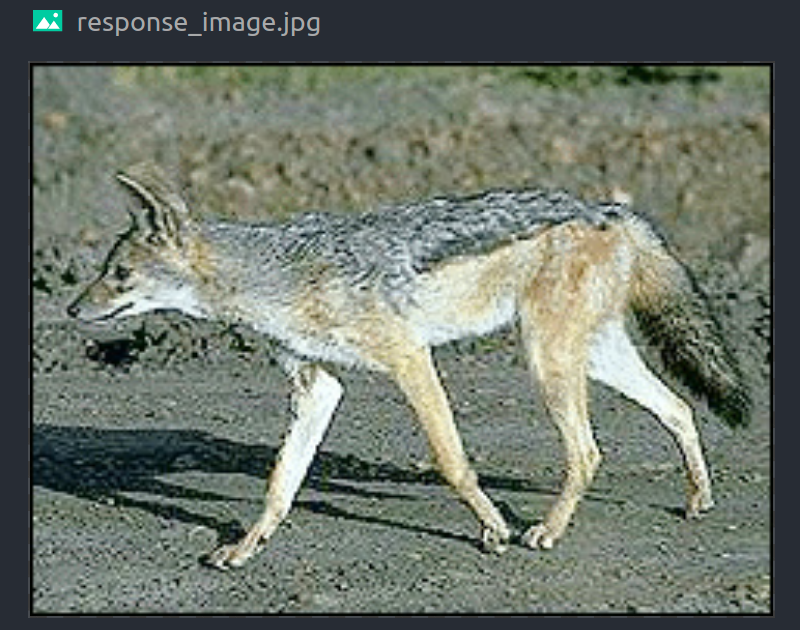
\includegraphics[width=0.6\textwidth]{get_request_output}
	\label{fig:get_request_output}
\end{figure}

More of the functionality that the library provides is demonstrated in the code snippet in \texttt{Figure \ref{fig:async_request_example}}. Here, the function \texttt{make\_request} is used to create a “DELETE” request over HTTPS. A header is added to specify the type of data to accept in the response from the server, using a string parameter. Four response callback types are supported by the library:
\begin{itemize}
	\item A raw progress callback can be set with the \texttt{Request::set\_raw\_progress\_callback} function and is called whenever one packet of (decrypted) data has been received from the socket. The callback takes a \texttt{ResponseProgressRaw} object which contains a reference to the data that has been received so far, an offset to the data that was just received, and a stop function to cancel any further receiving and processing of data.
	\item \texttt{Request::set\_headers\_callback} sets a callback that is invoked when the HTTP headers of the response have been received and parsed. The callback takes a \texttt{ResponseProgressHeaders} object which contains an interface for querying header data, a \texttt{ResponseProgressRaw} object, and a stop function. For example, if the user only wants the headers of the response and does not need to wait for the body to be received and parsed, this callback function can be used.
	\item \texttt{Request::set\_body\_callback} sets a callback that is invoked when a chunk of the body has been received and processed. The callback takes a \texttt{ResponseProgressBody} object which also has an interface to the previously received header data, a reference to the body data that was received so far, an optional total expected body size field that only holds a value if a \texttt{content-length} header was included in the response, a \texttt{ResponseProgressRaw} object and a stop function. An example use case of this callback is to provide user feedback in the form of a progress bar in a graphical user interface or to render what has been received so far of an image that is being retrieved from a website.
	\item \texttt{Request::set\_finish\_callback} sets a callback that is invoked when the full response has been received and parsed. It takes a \texttt{Response} object as a parameter.
\end{itemize}
In the example, the usage of a raw progress callback is demonstrated. The size of the data that has been received is written to the console. A lambda functor could have been used instead but a regular function was used in the example for added readability. The request is sent and the response is received asynchronously. A custom receive buffer size is specified as a template parameter to the \texttt{send\_async} function - if it was left as the default, all of the response data would be fetched at once and the output would not be as illustrative of the callback system. A message is written to the console while the response is received and the resulting response is awaited in the main thread. Lastly, the content-type header of the response is printed (or “Unknown” if there was no such header) and the full body data is printed as a string. \texttt{Figure \ref{fig:async_request_output}} shows a possible console output of the program.

\begin{figure}[hp]
	\centering
	\caption{Example library usage to perform an asynchronous, TLS encrypted “DELETE” request, using callbacks and printing the response body and content-type header value.}
	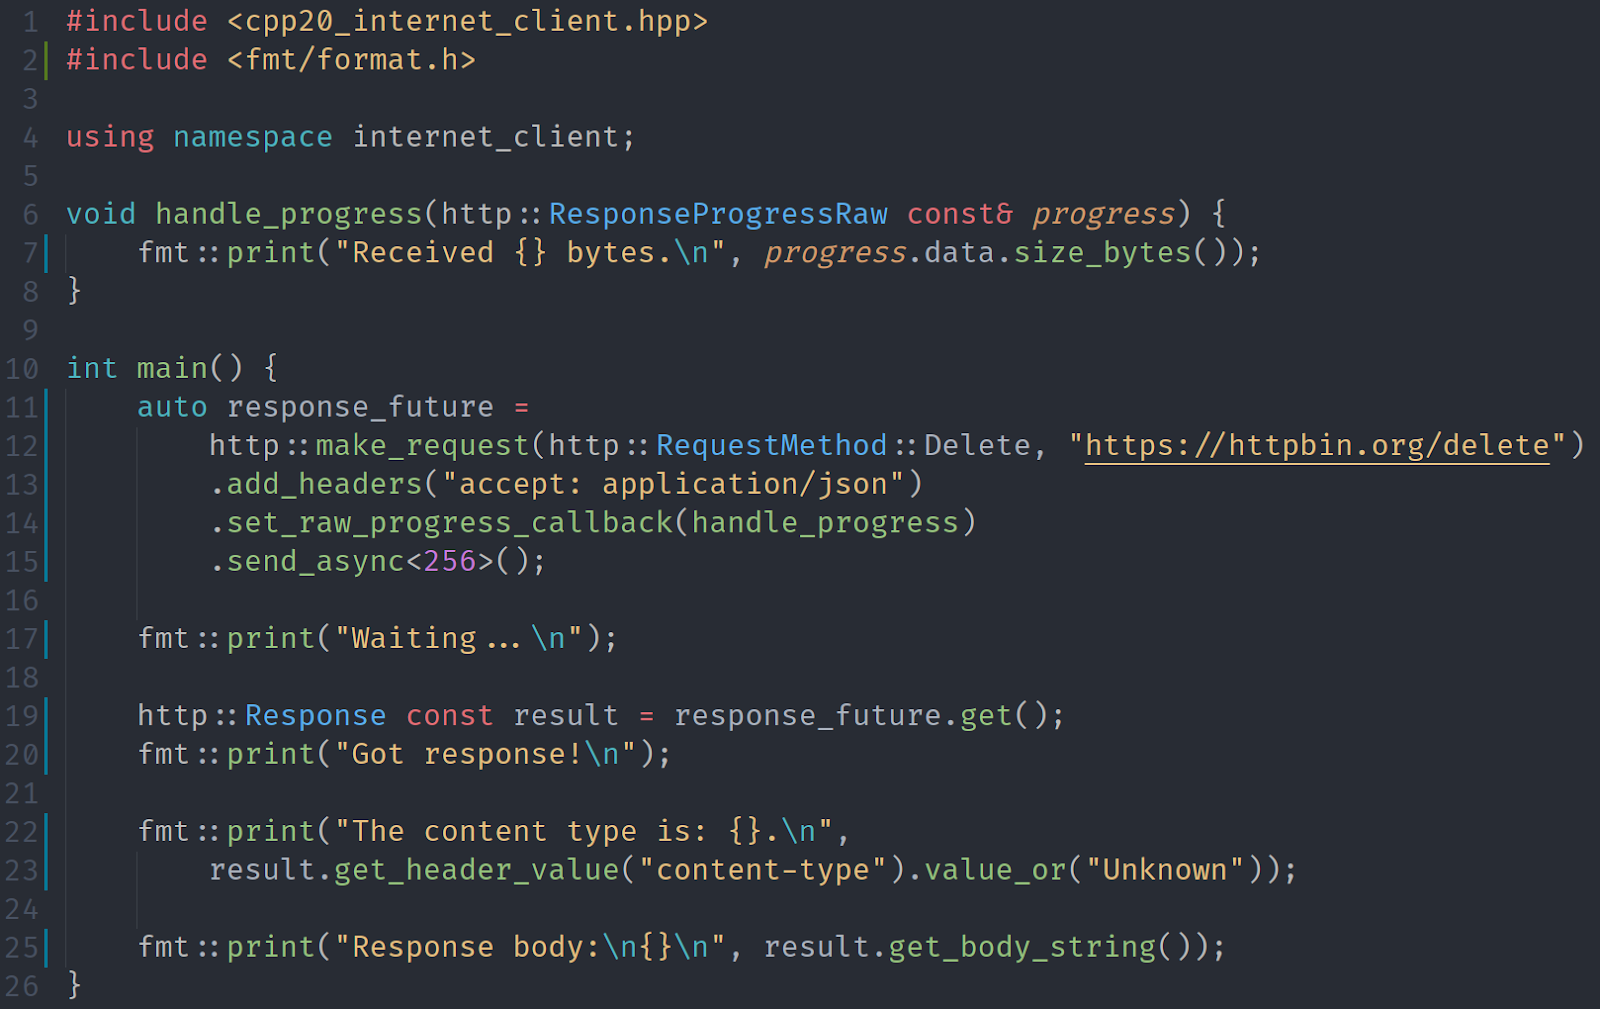
\includegraphics[width=\textwidth]{async_request_example}
	\label{fig:async_request_example}
\end{figure}

\begin{figure}[hp]
	\centering
	\caption{Possible console output of the program shown in Figure \ref{fig:async_request_example}}
	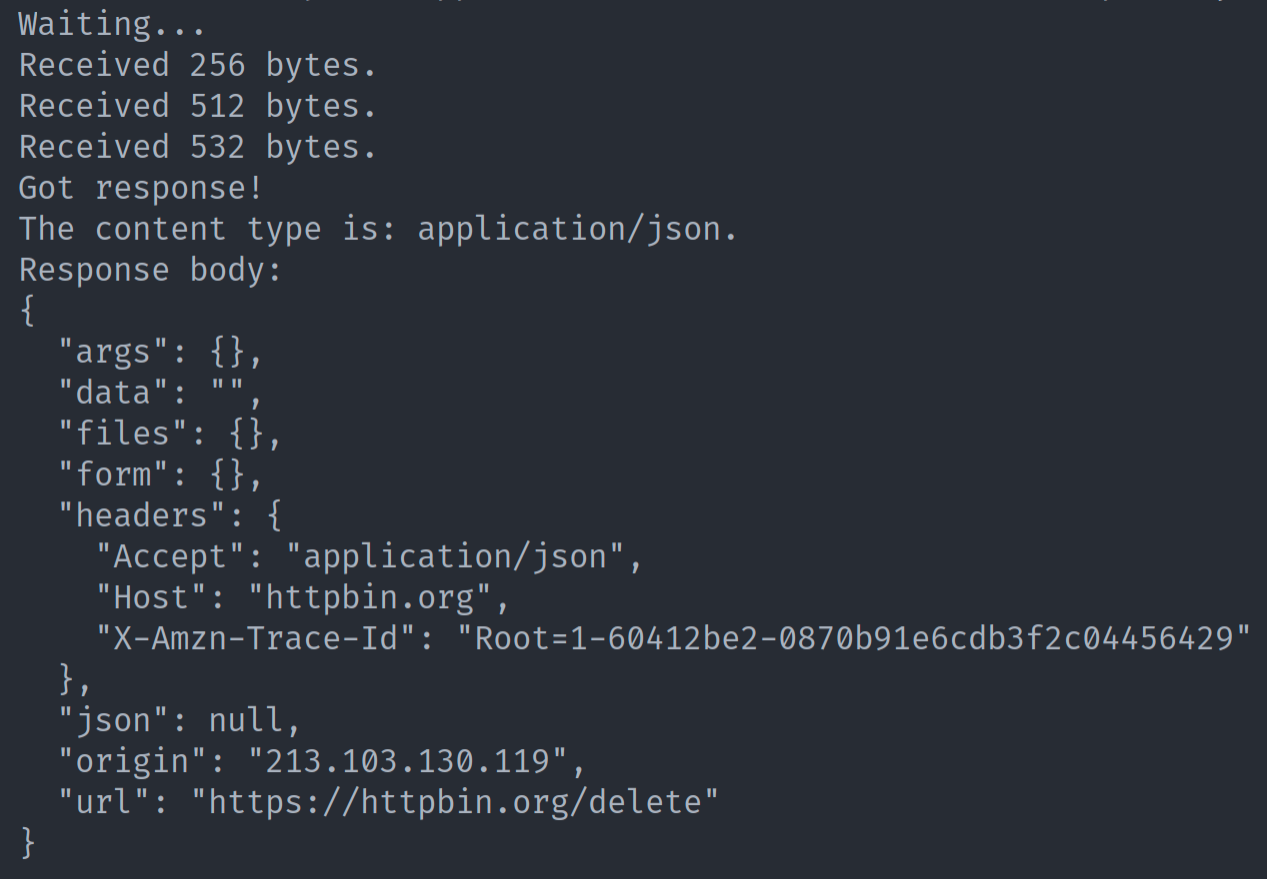
\includegraphics[width=0.8\textwidth]{async_request_output}
	\label{fig:async_request_output}
\end{figure}

\clearpage
\section{Discussion}
\subsection{Research methods}
The research methods were sufficient because I found the information that I required. I cannot think of any other suitable method of acquiring information for this project. Perhaps taking inspiration from a wider range of sources would lead to a different, potentially more ideal outcome, but this is not reasonably quantifiable.
\subsection{Work process}
The work process was functional and relatively efficient, although it could have been more structured. The test-driven development technique could have been followed more strictly, where development consists of cycles of first writing unit tests, then implementing the functionality and making sure the tests succeed. This was only done in some cases where it was known ahead of time exactly what the ideal usage of the interfaces would look like. The code was often instead designed with the future writing of unit tests in mind. This did make the code more modular than it would have been without any unit tests at all, and a lot of bugs were quickly eliminated instead of being discovered later in integration tests and through a more painful debugging process. The conclusion is that writing unit tests helped with the work process regardless.

Having a less structured work process meant that code was written in parallel with researching information and designing the architecture of the library. An alternative to this could have been starting with designing the architecture and then working in cycles of research and programming. In this project these three work processes were interdependent, so it is unclear whether following a more structured work process would benefit the result or the efficiency of the process.
\subsection{Software development process}
\subsubsection{Implementing HTTP}
Starting the software development on Windows was a disadvantage because of the large number of native networking APIs there were to choose from. It made it possible to use a native API that provided an implementation of HTTP, while there was no corresponding native API on Linux or MacOS. After realizing this, and researching about network sockets, a much better design and abstraction structure were made. Sockets are a basic building block that every operating system provides an API for. More specifically there is a POSIX socket API and a Windows socket API. These are very similar with even some functions having the same names and interfaces. 

This meant that I could make a \texttt{Socket} class that abstracts the only platform-dependent functionality in the whole library while building all other functionality on top of this, implemented in the header file in a cross-platform manner. This fits well with the way the communication protocols are stacked on top of each other; HTTP only needs an I/O stream to be implemented, and in this case, it is a TCP/IP socket that sends data in packets between a client computer and a server, optionally encrypted with TLS. 

Having to write the HTTP implementation from scratch was an interesting challenge and I learned a lot from designing the code for this. The hardest part was implementing the parser for the chunked Transfer-Encoding because the data is provided part-by-part in packets of varying sizes. The Single Responsibility Principle was kept in mind while designing the HTTP implementation.
\subsubsection{Adding TLS encryption}
There were multiple choices for implementing TLS encryption functionality. It was natural to abstract TLS encryption as part of the \texttt{Socket} class, having the option of either an unencrypted socket or an encrypted socket. Implementing TLS from scratch is very complex, as can be seen from the specification (\cite{TlsSpec}). It was discovered that there is a native API on Windows for TLS encryption called Schannel, and a corresponding cross-platform API called OpenSSL that is widely used for this purpose (\cite{OpenSSL}). Since OpenSSL must be made available on the system separately (although possibly with a C++ library manager like VCPKG), it is only used on Linux and MacOS. On Windows, it is more convenient to use the Schannel API since it is installed together with the Windows SDK. A large difference was noticed in the level of abstraction and ease of use of the two APIs. Implementing TLS encryption using Schannel was by far the hardest part of the whole project. 

An example that shows the difficulty in implementing TLS using Schannel was when a fixed size had to be determined for the TLS handshake message receive buffer. This buffer contains a piece of data, a message, received from the server during the handshake. A single function, \texttt{InitializeSecurityContext}, is called multiple times to perform a handshake (\cite{MicrosoftInitializeSecurityContext}). It takes one or more input buffers (most importantly, data received from the server to process) and returns one or more output buffers (most importantly, data to send to the server). The function takes twelve parameters in total, which in itself shows the complexity of interacting with the API.

The output buffer can be allocated by the function, but the input message buffer (data received from the server) needs to be allocated by the caller. Therefore, a maximum message size needs to be determined - unless there is a way to know if the message is incomplete and the buffer needs to be grown. According to the Microsoft documentation, the error code \texttt{SEC\_E\_INCOMPLETE\_MESSAGE} is returned if the input message buffer was too small to hold the complete message received from the peer. If this was the case, then the buffer could be grown and more data could be received from the socket, appending it to the buffer and calling the function again.

However, in practice, this was not true. Instead, the error code returned when an incomplete message was passed to the function was \texttt{SEC\_E\_INVALID\_TOKEN}. Trying to grow the buffer after getting that error code, calling the function again, and sending the output buffer to the peer causes it to close the connection when trying to read more data afterward. Therefore, a fixed size needed to be determined for the message buffer. It was not clear what this size would be. There is a function \texttt{QueryContextAttributes} for querying the TLS message header, message body, and trailer sizes, which would be perfect except for the fact that it only works after the secure connection is established (\cite{MicrosoftQueryContextAttributes}). 

The only thing the Microsoft documentation for \texttt{InitializeSecurityContext} tells us about the size of the message buffer is: “[...] the value of this parameter is a pointer to a buffer allocated with enough memory to hold the token returned by the remote computer.” (\cite{MicrosoftInitializeSecurityContext}). The TLS 1.3 standard specification says: “The record layer fragments information blocks into \texttt{TLSPlaintext} records carrying data in chunks of 2\^{}14 bytes or less." (\cite[][p. 78]{TlsSpec}). 

Looking at a few implementations of TLS encrypted sockets with Schannel:
\begin{enumerate}
	\item In an article from Microsoft’s documentation (\citeyear{SchannelUsageMicrosoft}), a sample program in C uses a maximum handshake message size of 12000 bytes.
	\item In a version of Chromium by Adobe, the maximum size is $5+16\cdot1024+64=16453$ bytes (\cite{SchannelUsageChromium}).
	\item In the source of the Curl library, the maximum size is $4096+1024=5120$ bytes (\cite{SchannelUsageLibcurl}).
	\item In the source of the GitHub repository “shells” by Odzhan (\citeyear{SchannelUsageOdzhanRepo}), the maximum size is 32768 bytes. This is $2^{15}$, which is twice as big as the maximum size of a \texttt{TLSPlaintext} record chunk.
\end{enumerate}

All of these implementations use different maximum handshake message sizes, which is quite interesting. I decided to follow the TLS specification and use $2^{14}$ = 16384 bytes as this is the maximum allowed size of any \texttt{TLSPlaintext} record block, which includes handshake messages (\cite{TlsSpec}). The buffer is then expanded after the handshake is complete to fit the message header and trailer using the return values of \texttt{QueryContextAttributes}.
\subsection{Results}\label{sec:Results}
\subsubsection{Programming paradigms}
According to the creator of C++ Bjarne Stroustrup (\citeyear{CppNotJustObjectOriented}), C++ is not an object-oriented programming language but supports multiple programming paradigms. This was taken advantage of in the project. Cpp20InternetClient uses functional, object-oriented, and generic programming paradigms both together and in different parts of the code to accomplish different goals. 

Most of the interfaces to the library are functional. For example, a form of currying is used to build requests. Requests are built in a sequence of function calls instead of with a single constructor taking many parameters. Requests are temporary objects, until for instance send has been called and the response object is returned. Furthermore, this response object is immutable and only queries about the response data can be made. Immutable data is also a characteristic of functional programming. Function composition and higher-order functions are also used, especially with the C++20 ranges library discussed in \textbf{\ref{sec:UsageOfFeatures}}.

Generic programming means making use of and writing generic functions and classes that are parametrized on types and/or objects at compile-time. In C++, the feature for this is called templates. Templates are a form of static/compile-time polymorphism, as a single interface is provided for multiple types (\cite{StaticPolymorphism}). The function call is determined depending on the template parameters at compile time. Function overloading is also an example of static polymorphism, where the types of parameters determine the function to call. Cpp20InternetClient makes extensive use of templates. For example, the majority of the functions and types in the \texttt{utils} namespace are templates, to make them generally applicable to any type that meets the minimum requirements for the type or function. To explicitly constrain these compile-time parameters, C++20 concepts are used. This is discussed further in \textbf{\ref{sec:UsageOfFeatures}}.

The project makes use of object-oriented techniques as well. Stroustrup (\citeyear{CppNotJustObjectOriented}) shows that object-oriented programming is characterized by having abstractions (classes and objects), being able to build upon existing abstractions (inheritance and composition), and making use of dynamic polymorphism (to look up function calls at runtime when interacting with pointers with the type of a base class or interface). To add to this description, it is often said that object-oriented objects contain mutable state, in comparison to objects in functional programming which are more often immutable. While the library makes no use of runtime polymorphism, it does make use of mutable objects and abstract class inheritance. 

An example of mutable objects is the \texttt{Socket} class, as functions for writing and reading data operate on a single instance. Something interesting about this is that even in a purely functional programming language like Haskell, sockets are object-oriented in a similar fashion (\cite{HaskellSocket}). I think this has to do with how the underlying socket API in C is designed, or with the concept of a socket in general - it might be hard to translate into a more functional interface. 

A better example of an object-oriented design in Cpp20InternetClient might be the parsing algorithms in the HTTP implementation, for example \\
\texttt{http::algorithms::ResponseParser}. This class has a single public member function \texttt{parse\_new\_data}, which takes a \texttt{std::span} of bytes (a reference to a data block) and returns a \texttt{std::optional<ParsedResponse>}, meaning it either returns nothing or a resulting parsed response. The class contains internal parsing state that is modified by the function, and once a full HTTP response has been parsed, the result is returned.

There is one example of inheritance in the library excluding the exception types. The abstract class \texttt{http::algorithms::ParsedHeadersInterface} is used to provide an interface to parsed header data for both the response and response progress classes; \texttt{Response}, \texttt{ResponseProgressBody}, and \texttt{ResponseProgressHeaders} (within the \texttt{internet\_client::http} namespace). The class does not contain any data members, but it contains default implementations of functions as well as a single virtual function for getting the \texttt{http::algorithms::ParsedResponse} object that its other functions query.
\subsubsection{Usage of C++ language and library features}\label{sec:UsageOfFeatures}
In this section, the usage of modern C++ language and library features in the project and their advantages are discussed. Only a select set of features are discussed here since very many new features are used.

In C++20, a language feature for modules was added to the standard. Making use of this feature would provide many benefits (\cite{AdvantagesOfCppModules}), but there is not yet full support for this feature in any compiler, nor in CMake. Therefore, the project is planned to make use of modules when the feature is well-supported. Another C++20 feature that the library does not make use of is coroutines (\cite{CppCoroutines}). It may have been possible to make use of them, but there is not yet enough support for them in the standard library and I had not done enough research about the feature to make use of it beyond writing a simple number generator.

C++20 introduces a new, more powerful, and simple way to constrain template parameters, called Concepts (\cite{CppConstraints}). This is in my experience the C++20 feature that has the largest impact on code. Before concepts, templates could be constrained in a hacky way using something referred to as SFINAE (Substitution Failure Is Not An Error) (\cite{CppSFINAE}). Because of the verboseness of SFINAE techniques to constrain template parameters, they were often left unconstrained. This meant that passing unsupported types as template parameters would result in very obscure compiler errors with references to code inside the template function that failed to compile with the specific type substitution for that template instantiation. With concepts, type requirements are part of the function declaration, which among other things enables more comprehensible and relevant compiler errors. Type constraints are also used by the compiler to select the most appropriate template specializations or function overloads.

In Cpp20InternetClient, all template parameters are constrained using Concepts, and the library defines its own set of concepts inside the \texttt{utils} namespace. One example of an application of Concepts in the library is shown in \textbf{Figure \ref{fig:constraints_example}}. Here they are used for an equality comparison operator that works for two different types of header objects; one that holds a copy of the header data (name and value strings) and one that holds string views that refer to data somewhere else. There are many syntax forms for specifying constraints, the form shown in \textbf{Figure \ref{fig:constraints_example}} is only one of them. The \texttt{IsHeader} concept evaluates to true for types that are either \texttt{HeaderCopy} or \texttt{Header}. It is defined using the \texttt{utils::IsAnyOf} concept shown in \textbf{Figure \ref{fig:is_any_of_concept}}, which uses a C++11 parameter pack and C++17 fold expression (\cite{CppFoldExpression}) to evaluate whether a type is equal to one of any number of types. Without templates and concepts, the code for the header comparison operator would have to be duplicated four times for all combinations of \texttt{HeaderCopy} and \texttt{Header} types.

C++20 also comes with a new functional “ranges” library (\cite{CppRanges}) as well as versions of the standard library algorithms that are constrained using Concepts, with overloads that take ranges instead of iterator pairs as parameters (\cite{CppConstrainedAlgorithms}). The name field of an HTTP header is case insensitive and only within the ASCII character set (\cite[][Section 4.2]{HttpSpec}). This is taken into account in the comparison operator, using the ranges library to compare the names case-insensitively. A transform is applied to both names that converts them to lowercase, and the constrained algorithm \texttt{std::ranges::equal} then compares them. The lowercase transform view is defined in \textbf{Figure \ref{fig:lowercase_transform_definition}}, using the lazily evaluated view and higher-order function \texttt{std::views::transform}. 

The library contains no usage of regular for-loops; only constrained algorithms, views, and range-based for loops are used. This makes the code more expressive, easier to understand and there is less space for bugs than the equivalent hand-written versions with “raw” for-loops (off-by-one errors, buffer overruns, signed/unsigned mismatches, integer over-/underflows, etc.). The performance cost of using these abstractions is small, as the compiler optimizes them well and all views are lazily evaluated. 

C++17 introduces a new \texttt{[[nodiscard]]} attribute for classes and functions, which makes the compiler warn about discarded values (\cite{CppNodiscard}). This attribute is applied to all pure functions for which it is with full certainty a mistake to ignore the return value. An example is any comparison operator, such as the one in \textbf{Figure \ref{fig:constraints_example}}. If two objects are compared without using the return value, it is with full certainty a mistake. There are places where the attribute has a bigger impact on making interfaces harder to use incorrectly. An example is \texttt{http::Request::send}. Being forced to use the return value makes the attempted usage of the function self-documenting; the result is not queried from the \texttt{Request} object, but rather the state is transformed into another interface in a functional fashion.

\begin{figure}[hp]
	\centering
	\caption{An example that shows usage of C++20 Concepts, standard ranges library, and the [[nodiscard]] attribute in the project.}
	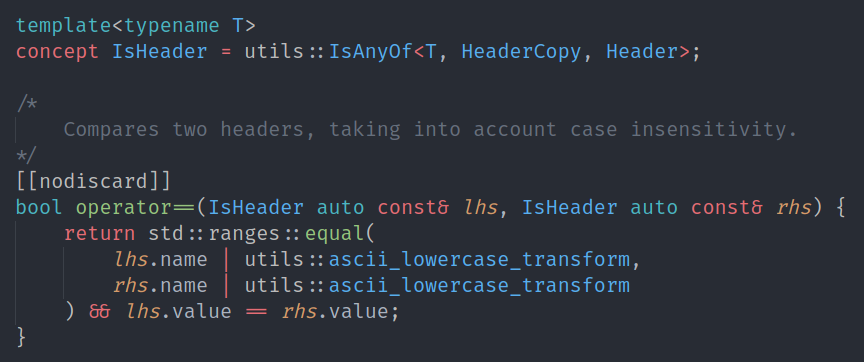
\includegraphics[width=\textwidth]{constraints_example}
	\label{fig:constraints_example}
\end{figure}

\begin{figure}[hp]
	\centering
	\caption{The definition of the \texttt{utils::IsAnyOf} concept, using C++17 fold expressions and C++20 \texttt{std::same\_as} concept.}
	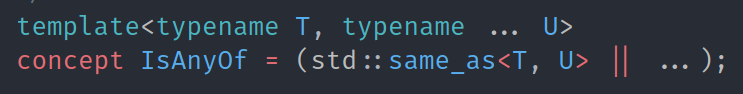
\includegraphics[width=0.8\textwidth]{is_any_of_concept}
	\label{fig:is_any_of_concept}
\end{figure}

\begin{figure}[hp]
	\centering
	\caption{The definition of \texttt{utils::ascii\_lowercase\_transform} using the \texttt{transform} view from the C++20 ranges library.}
	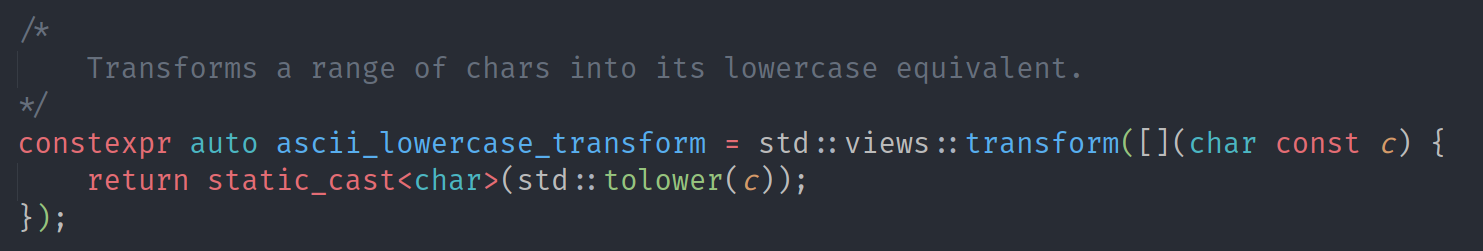
\includegraphics[width=\textwidth]{lowercase_transform_definition}
	\label{fig:lowercase_transform_definition}
\end{figure}

Another feature that is used as a way to enforce interfaces is reference-qualified member functions. Adding \texttt{\&\&} to the end of a member function declaration specifies that the object that the function is called on must be temporary (\cite{CppMemberFunctions}). This is used on all functions of the \texttt{http::Request} class. The data of a request object is moved once the request is sent, so the object should be discarded at that point. Adding the rvalue qualifier to the member functions enforces this.

In the C language, memory and other resources need to be freed/destroyed/closed manually with function calls, while C++ provides automatic resource management in the form of the perhaps unintuitively named RAII (Resource Acquisition Is Initialization) idiom (\cite{CppRAII}). RAII objects hold some resource that is automatically freed when the object goes out of scope. C++11 move semantics play a big part in this, as resources can be moved between objects efficiently without any allocations or deallocations. This allows the lifetime of resources to not be restricted to a single variable scope. All of the APIs that the library abstracts are written in C. To avoid the common bugs associated with manual resource management, RAII should be utilized with these APIs as well. There is a less-known feature in C++20 that is utilized heavily in the project to help with this: lambdas in unevaluated contexts (\cite{UnevaluatedLambdas}).

Using lambdas in unevaluated contexts, a new lambda type can be specified as a template parameter directly with the decltype keyword. This is utilized to easily designate a custom deleter for \texttt{std::unique\_ptr} types, as seen in \textbf{Figure \ref{fig:unevaluated_lambdas_unique_ptr}} where the function \texttt{BIO\_free} must be used to free BIO pointers in the OpenSSL API. Often in C APIs, a manually managed resource comes in the form of a “handle” that is an integer ID instead of a pointer. For these handles, a \texttt{std::unique\_ptr} cannot be used. Therefore, a similar type was written for arbitrary handle types and arbitrary “invalid handle” values, named \texttt{UniqueHandle}, in the \texttt{utils} namespace. \textbf{Figure \ref{fig:unique_handle_example}} shows an example of an instantiation of this class template to define a \texttt{SocketHandle} type for POSIX sockets. The first template argument is the underlying handle type, the second is the (required) custom deleter type and the third is the value used for invalid handles, which in this case is -1. These template parameters are constrained using C++20 Concepts, as shown in \textbf{Figure \ref{fig:unique_handle_constraints}}. The underlying handle must be trivial and the deleter must be an invocable that takes the handle type as a parameter. The third parameter does not have a type constraint as it is an object and not a type.

\begin{figure}[ht]
	\centering
	\caption{Usage of lambdas in unevaluated contexts to directly specify a custom deleter for a \texttt{std::unique\_ptr}.}
	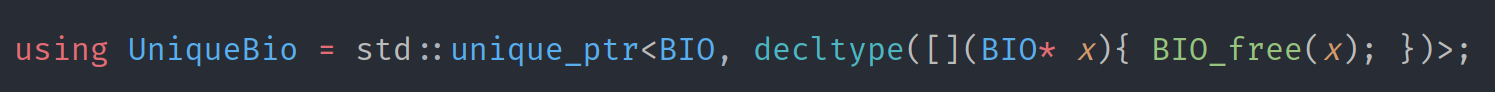
\includegraphics[width=\textwidth]{unevaluated_lambdas_unique_ptr}
	\label{fig:unevaluated_lambdas_unique_ptr}
\end{figure}

\begin{figure}[ht]
	\centering
	\caption{Example template instantiation for the \texttt{utils::UniqueHandle} class template.}
	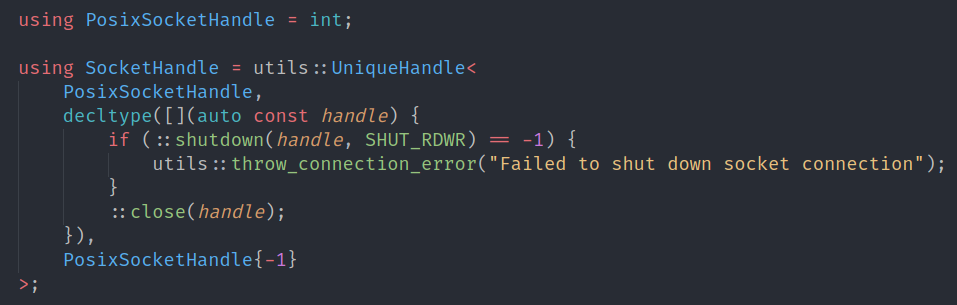
\includegraphics[width=\textwidth]{unique_handle_example}
	\label{fig:unique_handle_example}
\end{figure}

\begin{figure}[ht]
	\centering
	\caption{The type constraints for the \texttt{utils::UniqueHandle} class template.}
	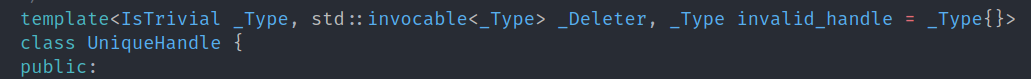
\includegraphics[width=\textwidth]{unique_handle_constraints}
	\label{fig:unique_handle_constraints}
\end{figure}

The C++ Core Guidelines (\cite{CppCoreGuidelines}) recommend avoiding passing pointers and lengths as separate parameters to functions taking a block of data or an array, which is very common in older code. Their suggested alternative is to use a span abstraction that holds these as data members. This type can also calculate the length automatically if constructed with an array or any other sized range, eliminating potential bugs from having to manually specify the length. In C++20, this type is added to the standard library. Cpp20InternetClient makes extensive use of \texttt{std::span} wherever a view over any contiguous data is needed. The \texttt{std::string\_view} type introduced in C++17 is similar to \texttt{std::span} but is used for immutable references to strings or parts of strings. The library also utilizes this type.

Common bugs in C++ programs stem from forgetting to initialize variables. The values of local objects that are not initialized and that do not have a default constructor that initializes them properly, like trivial types, are indeterminate (\cite{CppDefaultInitialization}). C++11 introduces the \texttt{auto} keyword for type deduction (\cite{CppAuto}). If the auto keyword is used in the declaration of a variable, it must be initialized. Prominent C++ expert Herb Sutter (\citeyear{AlmostAlwaysAuto}) advocates the use of the Almost Always Auto (AAA) style and presents good reasons to follow it, the strongest being that it is impossible to forget the initialization of variables. Using the AAA style also means that all local variables are declared with the type on the right-hand side of the declaration. 

When this style was first adopted, it had some drawbacks that made it undesirable in cases where the type has an expensive move constructor, and impossible if it has no move/copy constructors at all. Since C++17, copy/move construction is required to be elided in certain cases (\cite{CppCopyElision}). This made both initialization styles in \textbf{Figure \ref{fig:auto_type_deduction}} equivalent; Type is not required to have a move or copy constructor anymore. Therefore, there are no drawbacks to using this style today. The only place where \texttt{auto} is not used in local variable declarations in the project is when the intention is to initially leave the variable uninitialized, perhaps because it is immediately initialized by a function from a C API.

\begin{figure}[ht]
	\centering
	\caption{Two variable initialization styles that are required to be equivalent since C++17.}
	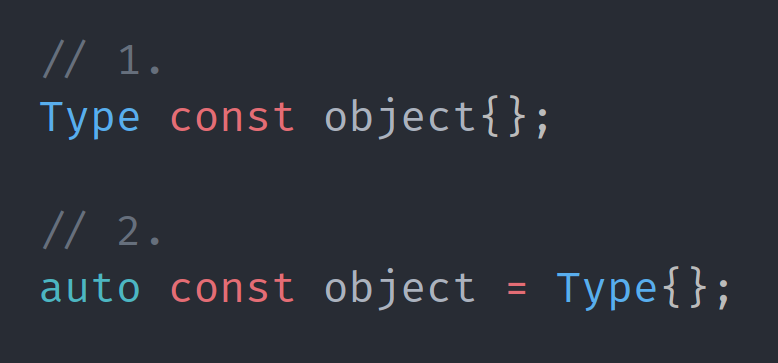
\includegraphics[width=0.5\textwidth]{auto_type_deduction}
	\label{fig:auto_type_deduction}
\end{figure}

\subsubsection{Error reporting and handling}
The C++ Core Guidelines (\cite{CppCoreGuidelines}) recommend using exceptions instead of error codes for reporting errors and provides strong reasons for doing so. Therefore, the library uses exceptions to report errors to the user. The namespace \texttt{internet\_client::errors} contains a collection of error types that are thrown by the library. This collection is very small, there are only two error types. These are \texttt{ConnectionFailed} and \texttt{ResponseParsingFailed}, and they inherit from \texttt{std::exception} to conform to the same common interface that all standard library exceptions conform to. \texttt{std::exception} only has a virtual what function that returns a description of the error. 

\texttt{ConnectionFailed} is thrown whenever an error code is reported by the underlying socket API or TLS API. The class contains a public member function \texttt{get\_is\_tls\_failure} which indicates whether the error comes from the TLS API or the socket API. An alternative to this could be to have separate error types for TLS errors and TCP/IP socket errors, but having a single error type makes the interface simpler in the most common case where this distinction is not required. 

\texttt{ResponseParsingFailed} should never be thrown if a request is made to a server that conforms to the HTTP/1.1 specification. However, this type is still provided since there are separate modules for parsing response data. These could still be given invalid input if used separately, so the error type is provided.

\subsubsection{Performance}
Most of the runtime of an HTTP request is spent sending and receiving data over the network. This makes performance improvements to most of the code irrelevant in practice. However, thought was put into things like minimizing unnecessary copying of data. If a large amount of data is received from the peer, a performance hit may be noticed if it is copied many times, in the parsing algorithms for instance. As mentioned in \textbf{\ref{sec:UsageOfFeatures}}, \texttt{std::span} is utilized whenever possible and safe to pass around mutable and immutable references to blocks of data instead of potentially copying. Similarly, \texttt{std::string\_view} is used for immutable references to strings or parts of strings. General best practice rules such as passing small objects by value to avoid unnecessary indirections, marking objects const if they are not mutated, and using move semantics (\cite{CppCoreGuidelines}) were followed even if the total performance difference has not been measured and might or might not be significant. Many of these practices benefit both performance and safety, so there was no reason not to follow them.

\subsubsection{Safety}
Many, if not all of the language and library features discussed in \textbf{\ref{sec:UsageOfFeatures}} improve safety and reduce bugs in some way. Old features are also reaching their full potential for safety in newer standards. Being able to use RAII easily with arbitrary C APIs (thanks to lambdas in unevaluated contexts) makes memory leaks and use-after-free errors impossible. I have observed that the ISO C++ standards committee puts a high priority on features that can contribute to the safety and performance of programs. Following new best practices that rely on these features, I have noticed how much less time and effort I have been spending on debugging runtime errors - and how much more time I have been spending on compile-time errors, compared to my previous development. In my view, this is a very positive change. Taking advantage of the compiler to save the developer early is better than searching every corner of a large jungle later on just to find a small use-after-free error that crashed the program. 

\subsubsection{Testing}
Putting effort into writing extensive unit tests is also something that can save the developer early. To make unit testing as effective as possible, all non-trivial functionality that can be tested as a unit/component should be tested. It was found that following the Single Responsibility Principle helped with this. By breaking up functionality into smaller modules that have their own responsibilities and are loosely coupled, they can be individually tested with ease. 

The only code that is not unit tested is the \texttt{Socket} and \texttt{Request} classes, and a few functions that depend directly on these. This is because of three reasons:

\begin{enumerate}
	\item They are abstractions of APIs which we have no control over, so testing them would not only test the abstraction layer but rather mostly the underlying API.
	\item As a consequence of the previous point, writing reliable tests for these components would be next to impossible. The internet is inherently unreliable. A server that we know the exact behavior of would have to be written and a synthetic internet connection would need to be mocked, if not the whole socket API.
	\item Sending data over the internet takes time, and unit tests are meant to be quick, especially because of their large quantity.
\end{enumerate}

Instead of doing that, these components were tested in a form of integration tests, which in this case was by writing the example programs located in the examples directory and testing them with different servers. The components that cannot be unit tested should be kept as thin as possible, extracting any unit-testable functionality into separate functions and classes.

\clearpage
\section{Conclusions}
One conclusion that can be drawn is that modern C++ features introduced in recent years provide more capable tools for writing stronger interfaces, safer code, and overall can reduce the time spent debugging runtime errors. However, features are only tools, and they can be used in many ways. Having new, well-designed features does not by itself improve the quality of software. To write Good Code™, especially in such a backward-compatible programming language, a carefully selected set of guidelines is still required and thought needs to be put into software design. The C++ Core Guidelines have proven, at least in this work, to give positive results.

Designing a good abstraction structure for the library was a challenging task, especially because the abstraction structure to a large degree was dependent on which low-level APIs the library was built upon. A conclusion from the development of this work is that it is a good idea, in cross-platform projects built on native APIs, to put thought into choosing the APIs to abstract early on in the process, perhaps by looking for the lowest common denominator among the platforms you are wishing to support. In this case, sockets were the lowest common denominator.

Cpp20InternetClient was admittedly the first project that I wrote unit tests for. Thought was put into separating functionality into modules that have their own responsibilities, with separate, simple interfaces, as this made the modules easier to test separately. It can be concluded that good test coverage can be accomplished by following the Single Responsibility Principle and extracting as much functionality as possible from modules that cannot be unit tested. A good guideline is to keep functions and classes small.

I look forward to seeing how C++20 modules will affect software development in the future, as moving from header files and implementation files to modules will change the way we write code and structure our projects. I am also curious about how coroutines will be utilized in future projects when the standard library has strong support for them.

\clearpage
\printbibliography

\end{document}